%! Author = jonathan
%! Date = 5/27/25
\chapter{Method}\label{ch:method}
\begin{figure}[!ht]
    \centering
    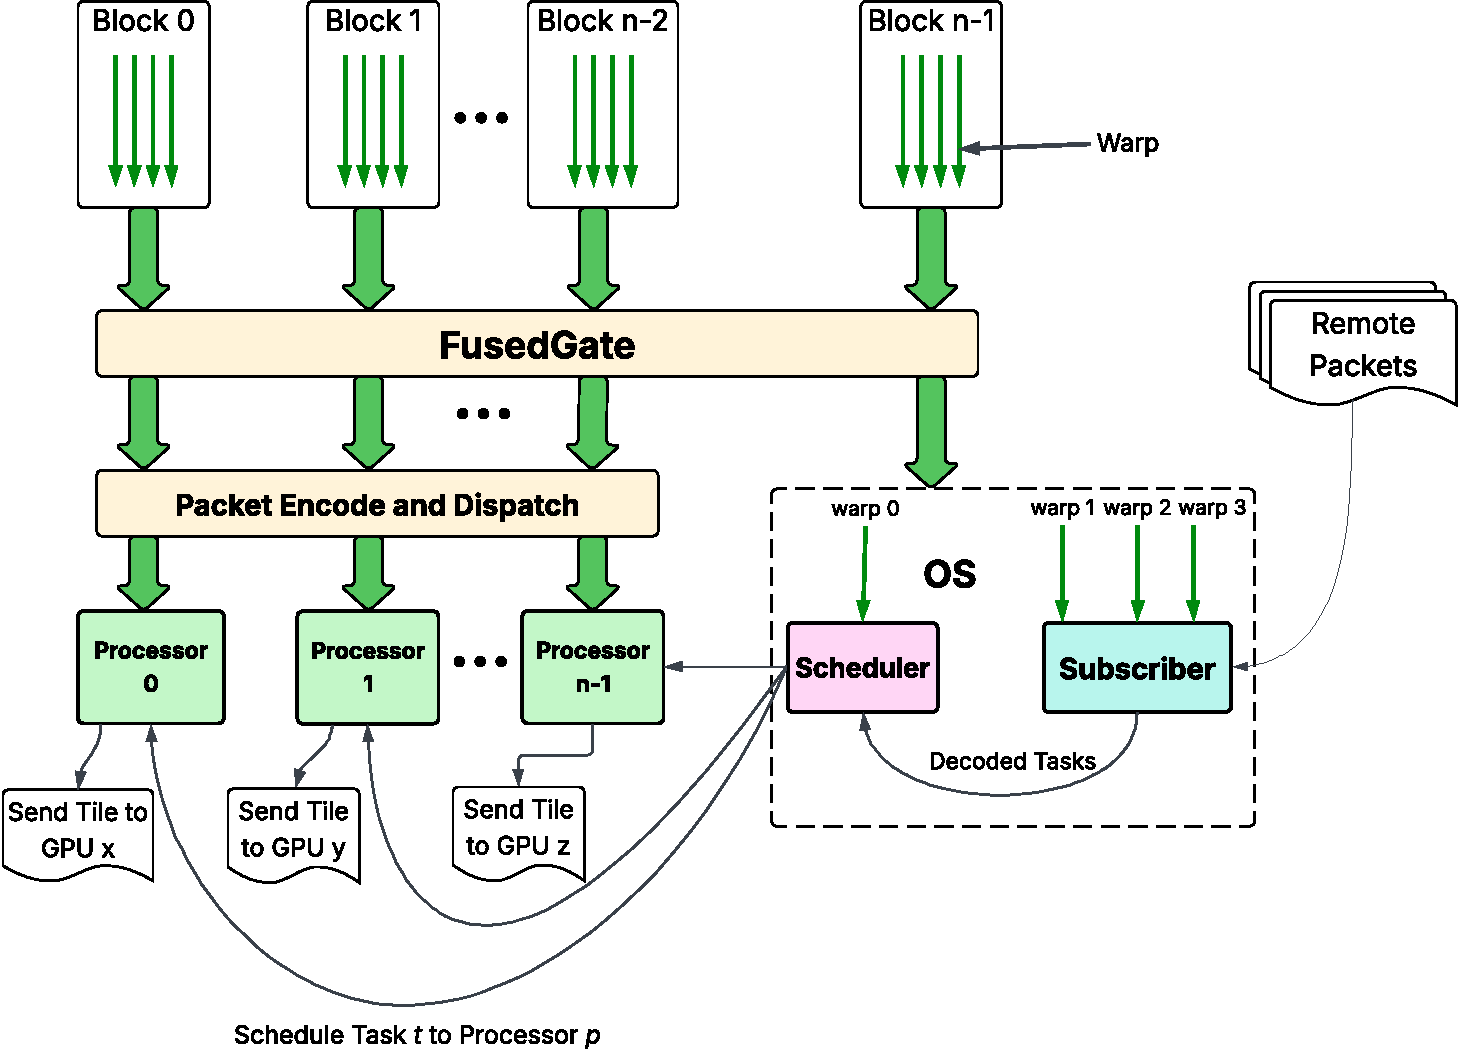
\includegraphics[width=0.8\textwidth, keepaspectratio]{figures/architecture}
    \caption{\emph{\sysname Fused Kernel}. Green arrows demonstrate block or warp specialization.}
    \label{fig:fusedK}
\end{figure}
Modern distributed MoE systems suffer from two limitations: (1) frequent many-to-many
(\emph{AlltoAll or AllGather}) collectives on the critical path, and
(2) significant overhead from repeated kernel launches.
We address these in \sysname, a fully fused MoE operator implemented
as a single persistent GPU kernel.
Unlike previous approaches~\cite{comet, deepep, pmlr-v162-rajbhandari22a, megatron, MLSYS2023_5616d34c,
    MLSYS2024_339caf45, 10.1145/3503221.3508418, 10.1145/3588964, 10.1145/3627703.3650083, 10.1145/3710848.3710868,
    NEURIPS2022_67d57c32},
\sysname is the first solution to implement a \emph{completely fused Distributed MoE kernel},
eliminating kernel launch overhead entirely by requiring only a single kernel launch (see Table~\ref{tab:gpuOps}).

\SetKwInput{KwRequire}{Require}
\SetKwInput{KwResult}{Result}
\SetKwInput{KwInput}{Input}
\SetKw{kwAnd}{and}
\SetKw{kwOr}{or}
\SetKw{kwTrue}{True}
\SetKw{kwFalse}{False}
\begin{algorithm}[!h]
    \small
    \DontPrintSemicolon
    \caption{~\emph{\sysname Distributed MoE Fused Kernel}}\label{alg:one}
    \KwInput{$A, O \in \mathbb{R}^{S\times H},\; X \in \mathbb{R}^{E\times H \times D},\; N$}
    \Begin{
        $T_{\phi}, G_{\phi} \gets \mathbf{FusedGate}(A)$\;
        \eIf{$\text{blockId} + 1 < N$}{
            $\mathbf{Dispatch}(T_{\phi}, A)$\;
            processor::start()\;
        }{
            \eIf{$warpID == 0$}{
                scheduler::start()\;
            }{
                subscriber::start($T_{\phi}$, $G_{\phi}$, $O$, $X$)\;
            }
        }
    }
\end{algorithm}
\begin{figure}[!ht]
    \centering
    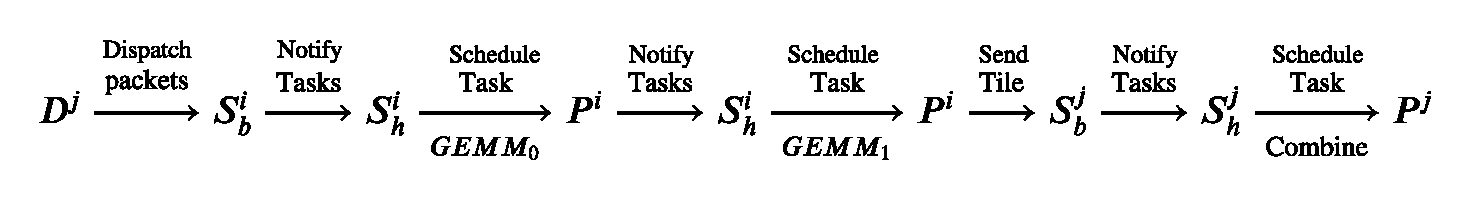
\includegraphics[width=\linewidth]{figures/actors}
    \caption{\emph{DMoE Functional Dependencies Expressed as a Chain of Actor Interactions}.
    We denote $S_b$, $S_h$, and $P$ as the
    Subscriber, Scheduler and Processor actors, respectively. For any actor $a \in \{S_b,\>S_b,\>P\}$,
        $a^i$ identifies an actor on GPU $i$. We define $D^j_i$ as the operator,
        where GPU $j$ dispatches packets of tiles to GPU $i$,
        This diagram expresses task dependencies at the granularity of a tile, namely
        $GEMM_0$, $GEMM_1$, combine and communication produce an output tile.
        Notifications occur as signals propagated through shared memory (subscriber $\leftrightarrow$ scheduler) or
        global memory (scheduler $\leftrightarrow$ processor or inter-GPU communication). Note one-sided
        inter-GPU transfers (packet or single tile) are \emph{coupled} with a signal to
        notify $S_b^j$ on the receiving GPU $j$ of the message's delivery.
    }
    \label{fig:actors}
\end{figure}
\section{Actor Model}\label{sec:actor-model}
The design of \sysname is based on the actor model of concurrent
computation~\cite{agha:85, 10.5555/1624775.1624804, Greif:75}.
We implement this model by specializing GPU thread blocks and warps into three distinct actor roles:
(1) \textbf{Processor} (\S\ref{alg:processor}), (2) \textbf{Subscriber} (\S\ref{alg:susbcriber}),
and (3) \textbf{Scheduler}(\S\ref{alg:scheduler}).
The Processor performs compute (GEMMs and element-wise operations) and tile communication.
We use CUTLASS~\cite{Thakkar_CUTLASS_2023} as the underlying infrastructure for high-performance
BLAS routines and NVSHMEM for kernel-initiated communication~\cite{nvshm}.
The Subscriber and Scheduler perform administrative functions.
Specifically, the Scheduler assigns computational tasks to available thread blocks.
Our key innovation is making the Scheduler both \emph{multithreaded},
enabling high scheduling throughput, and \emph{work-conserving}, ensuring consistently high GPU SM utilization.
On the other hand, the Subscriber decodes \emph{tile packets} from peer GPUs to task descriptors
(\S\ref{sec:task}).
Of the $N$ thread blocks on a GPU, we specialize $N-1$ to adopt the \textbf{Processor} role.
We specialize the last block as the Operating System (OS).
Within this block, we specialize three warps for the \textbf{Subscriber} role and
one warp for the \textbf{Scheduler} role.
This split of thread blocks across actors is intentional: our goal is to use few resources for administrative
tasks while reserving bulk of the resources for performing MoE computation tasks.
Figure~\ref{fig:fusedK} summarizes the
\sysname architecture and its constituent actors, while Algorithm~\ref{alg:one} gives a very close translation of the
system in code.
Note that $A \in \mathbb{R}^{S \times H}$ is the input token matrix;
$O \in \mathbb{R}^{S \times H}$ the output matrix;
and $X \in \mathbb{R}^{E\times H \times D}$ is a 3-D tensor of expert weights,
where $E$ denotes the number of local experts for the executing GPU, $H$ is the embedding dimension,
$D$ is the FFN intermediate dimension and $S$ is the sequence length.
$T_{\phi} \in \left(\mathbb{R}^2\right)^{E \times C}$
is a routing table data structure, where $T_{\phi}\left( e, c\right) = (i, w)$ indicates that token $i$ at slot $c$
dispatches to expert $e$. $w$ is the combine weight (Equation~\ref{eq:combine1}) and $C$ is expert capacity.
The tuple structure of $T_{\phi}$ is an implementation detail. $G_{\phi} \in \mathbb{R}^{S \times E}$ captures
the affinity scores produced by the gate (Equation~\ref{eq:combine2}).
\section{Inter-Actor Interactions}\label{sec:inter-actor-interactions}
\begin{figure}[!ht]
    \centering
    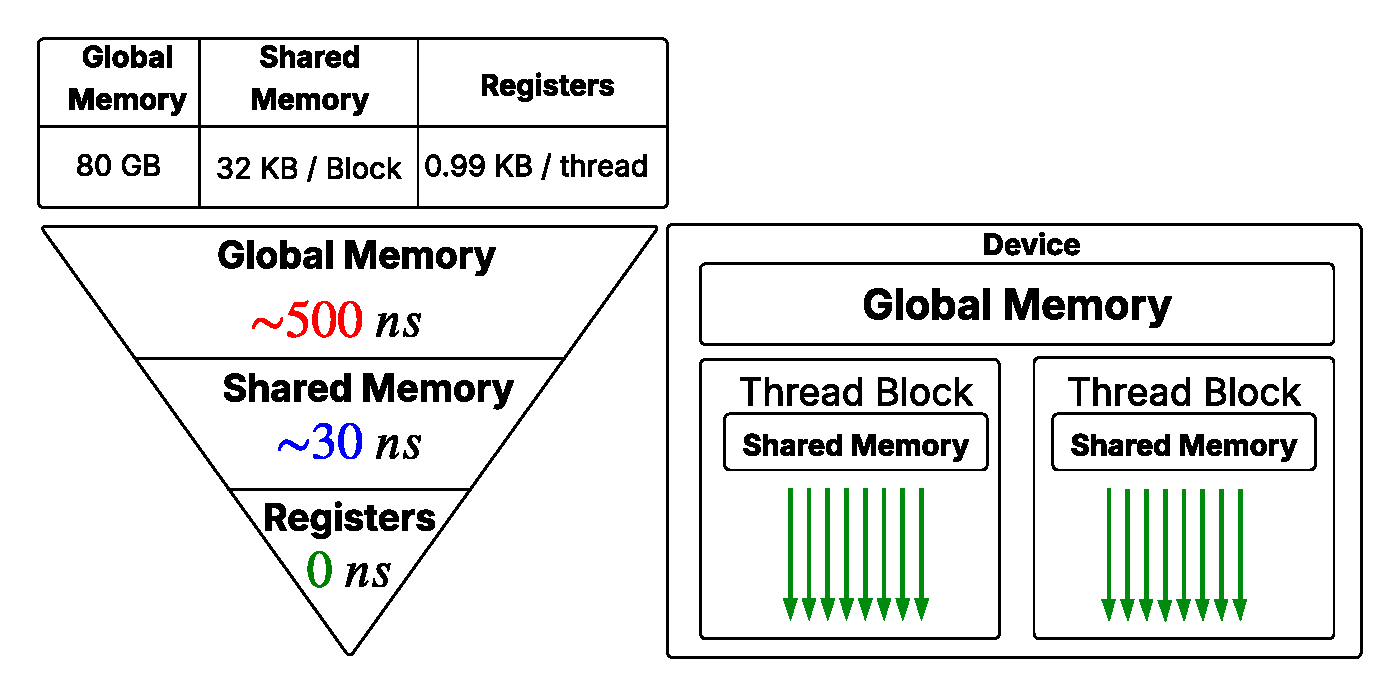
\includegraphics[width=4in, keepaspectratio]{figures/mem}
    \caption{\emph{GPU Memory Hierarchy}.
    The inverted pyramid (left) shows the load/store access latency~\cite{10579250, amperearch, ptx}. Table above outlines the capacity for different memory tiers (for A100 GPUs). The shared memory and register capacity are static configurations for \sysname.
    The right figure shows accessibility scopes: on-chip \textbf{registers}
    are scoped to a thread; on-chip \textbf{shared memory} is visible to all threads in a block;
    and off-chip \textbf{global memory} is accessible by all threads on device.}
    \label{fig:mem}
\end{figure}
\sysname decomposes MoE computation and communication at the granularity of a tile, a statically sized partition of a tensor,
to achieve parallel execution and efficient overlap of tasks.
Each tile maps to a discrete unit of work encapsulated by a \emph{task descriptor}.
The \textbf{Subscriber} decodes these task descriptors from the remote tile packets it receives.
Concurrently, the \textbf{Scheduler} receives notifications about available tasks and dispatches them for execution
to \textbf{Processor} actors that perform computations defined by these tasks,
namely the feed-forward network (FFN) and expert-combine operations.
Figure~\ref{fig:actors} show the chain of actor interactions, demonstrating how \sysname
enforces DMoE functional dependencies.
\section{Tiling}\label{sec:tiling}
Selecting appropriate tile dimensions in \sysname is crucial to ensure efficient GPU utilization.
An undersized tile underutilizes the GPU,
while excessively large tiles create register pressure,
causing performance-degrading register spills to local memory.
After careful parameter sweeps,
we choose tile dimensions of (128, 64).
Our key insights are: increasing tile width significantly raises the register usage per thread,
potentially triggering costly spills;
increasing tile height without adjusting thread count increases workload per thread, harming performance.
Raising the thread count per block beyond our fixed value of 128 threads reduces the number of concurrent blocks,
negatively affecting SM occupancy.
Larger thread-block sizes also increase overhead from intra-block synchronization (\emph{\_\_syncthreads()} barriers),
further degrading performance.
Thus, our chosen tile dimensions balance register usage, shared-memory constraints,
and GPU occupancy to deliver optimal performance.
\begin{algorithm}[!ht]
    \DontPrintSemicolon
    \SetKwBlock{DoParallel}{do in parallel}{end}
    \SetKwInput{KwInput}{Input}
    \KwInput{$T_{\phi} \in \left(\mathbb{R}^2\right)^{E \times C}$, $G_{\phi} \in \mathbb{R}^{S \times E}$
        $O \in \mathbb{R}^{S \times H}$, $X \in \mathbb{R}^{E\times H \times D}$}
    \caption{~\emph{Subscriber Actor}: executed by three warps}\label{alg:susbcriber}
    \Begin{
        $interrupt \gets \mathbf{GetSharedInterrupt}()$\;
        $flags \gets \mathbf{GetSymmetricFlags}()$\;
        $tQ \gets \mathbf{GetTQ}()$\;
        \tcp{Predefined upper bound on the number of tasks.}
        \tcp{Modulated to the actual task count computed}
        \tcp{from dispatch signals received from peer GPUs}
        $taskBound \gets \mathbf{GetTaskBound}()$\;
        \While{$\mathbf{AtomicLoad}(interrupt) == $ \kwFalse}{
            \tcp{dispatch flags}
            \DoParallel{
                Visit dispatch flags\;
                Atomically retrieve signal\;
                \If{Signal is set and flag is not visited}{
                    Mark visited\;
                    $\mathbf{SelfCorrectTaskBound}(taskBound, Signal)$\;
                    Enforce memory consistency before consuming packet\;
                    Decode packet into a set of $GEMM_0$ task descriptors\;
                    Write task descriptors to $tQ$\;
                    Notify Scheduler of decoded tasks\;
                }
            }
            Advance flags by number of dispatch flags length\;
            Atomically retrieve signal\;
            \tcp{combine signals}
            \DoParallel{
                Visit combine flags: one per tile\;
                \If{Signal is set and flag is not visited}{
                    Mark visited\;
                    Enforce memory consistency before consuming packet\;
                    Decode packet into a set of $combine$ task descriptors\;
                    Write task descriptors to $tQ$\;
                    Notify Scheduler of decoded tasks\;
                }
            }
        }
    }
\end{algorithm}
\begin{algorithm}[!ht]
    \DontPrintSemicolon
    \SetKwInput{KwInput}{Input}
    \SetKwBlock{DoParallel}{do in parallel}{end}
    \caption{~\emph{Scheduler Actor}: executed by one warp}\label{alg:scheduler}
    \Begin{
        $scheduled \gets 0$\;
        $tTB \gets 0$\;
        $tqS \gets \{\}$\;
        $pTDB \gets \mathbf{GetProcessorDoorbell}()$\;
        $sTDB \gets \mathbf{GetSubscriberDoorbell}()$\;
        $taskBound \gets \mathbf{GetTaskBound}()$\;
        $tTB \gets \mathbf{AtomicLoad}(taskBound)$\;
        \tcp{circular buffer ready queue}
        $rQ \gets \{\}$\;
        \tcp{Populate ready queue with Processor ids}
        $\mathbf{PopulateRQ}(rQ)$\;
        \While{$scheduled < tTB$}{
            $lt \gets 0$\;
            \DoParallel{
                Sweep doorbells and populate task counts into $tqS$\;
                Aggregate locally observed task counts into  $lt$\;
            }
            $qS,\>taskTally \gets 0$\;
            \tcp{qS is the inclusive output}
            $\mathbf{WarpInclusiveSum}(lt, qS, tasktally)$\;
            \While{$tasktally > 0$}{
                Repopulate $rQ$ with ready processor ids \;
                \DoParallel{
                    Starting at $rQ[qS]$ signal processors about tasks from $tqS$
                }
            }
            \If{$threadId == 0$}{
                $tTB \gets \mathbf{AtomicLoad}(taskBound)$\;
            }
            $tTB \gets \mathbf{WarpBroadcast}(tTB)$
        }
        $\mathbf{InterruptSubscribers}()$\;
        $\mathbf{InterruptProcessors}()$\;
    }
\end{algorithm}
\begin{algorithm}[!h]
    \DontPrintSemicolon
    \caption{~\emph{Processor Actor}: executed by a block}\label{alg:processor}
    \Begin{
        $tQ \gets \mathbf{GetTQ}()$\;
        $signal \gets 0$\;
        \tcp{shared memory variables}
        $task \gets \{\}$\;
        $interrupt \gets \kwFalse$\;
        $complete \gets \kwFalse$\;
        \While{$interrupt == $ \kwFalse}{
            \If{$warpId == 0$}{
                \If{$threadId == 0$}{
                    $\mathbf{awaitTaskFromScheduler}(interrupt,\>signal)$\;
                    $\mathbf{FencedNotifyRQ}(ready)$\;
                }
                $\mathbf{syncwarp}()$\;
                $\mathbf{warpReadTQ}(tQ, \>signal, \>task)$\;
            }
            $\mathbf{syncthreads}()$\;
            \If{$interrupt == $ \kwFalse}{
                \Switch{task.Type}{
                    \Case{$GEMM_0$}{
                        \tcp{fused GEMM, epilogue and async tile staging}
                        $\mathbf{fGET}(GEMM_0, \>task)$\;
                        \If{$threadId == 0$}{
                            $complete \gets \mathbf{NotifyTileCompletion}()$\;
                        }
                        $\mathbf{syncthreads}()$\;
                        \If{$complete == \kwTrue$}{
                            $\mathbf{NotifySchedulerNextGEMM}(tQ)$\;
                        }
                    }
                    \Case{$GEMM_1$}{
                        \tcp{fused GEMM, epilogue and async tile transfer}
                        $\mathbf{fGET}(GEMM_1, \>task)$\;
                    }
                    \Case{$Combine$}{
                        $\mathbf{combine}(task)$\;
                    }
                }
            }
        }
    }
\end{algorithm}